% Created 2024-09-17 ma. 11:47
% Intended LaTeX compiler: pdflatex
\documentclass[aspectratio=169, usenames,svgnames,dvipsnames]{beamer}
\usepackage[utf8]{inputenc}
\usepackage[T1]{fontenc}
\usepackage{graphicx}
\usepackage{longtable}
\usepackage{wrapfig}
\usepackage{rotating}
\usepackage[normalem]{ulem}
\usepackage{amsmath}
\usepackage{amssymb}
\usepackage{capt-of}
\usepackage{hyperref}
\usepackage{color}
\usepackage{listings}
\usepackage[spanish]{babel}
\setbeamercolor{alerted text}{fg=Blue}
\setbeamerfont{alerted text}{series=\bfseries}
\setbeamercolor{block title}{bg=structure.fg!20!bg!50!bg}
\setbeamercolor{block body}{use=block title,bg=block title.bg}
\AtBeginSubsection[]{\begin{frame}[plain]\tableofcontents[currentsubsection,sectionstyle=show/shaded,subsectionstyle=show/shaded/hide]\end{frame}}
\AtBeginSection[]{\begin{frame}[plain]\tableofcontents[currentsection,hideallsubsections]\end{frame}}
\lstdefinelanguage{R}{
  alsoletter={., <-},
  morekeywords={calcSol, calcG0, calcGef, prodGCPV, prodPVPS, calcShd, optimShd, Meteo2Meteo, readBDd, 
    readG0dm, readSIAR, corrFdKt, fBTd, fCompD, fCompI, fInclin, fProd, fPump, fSolD, fSolI,
    fSombra, fTemp, fTheta, HQCurve, local2Solar, NmgPVPS, sample2Diff, solarAngles, zoo2Meteo,
    show, shadeplot, xyplot, summary, rbind, c, download.file, dt2Meteo, read.csv.zoo,
    function, list, data.table, as.data.tableD, as.data.tableI, compare, print, S3method,
    import, exportClasses, exportMethods, importClassesFrom, importMethodsFrom, library, readBDi,
    fBTi, <-, profvis, median, format, missing, switch, is.list, switch, modifyList, do.call,
    markovG0, indexD, indexI, as.Date, cumsum, mean, sum, DOM, new, return, setcolorder,
    stopifnot, warning, as, is.data.frame, as, class, getData, paste, paste0, lapply,
    month, year, P2E, abs, is.data.table, attr},
  morekeywords=[2]{TRUE, FALSE, NULL, solaR.theme, if, else, with},
  sensitive=true, % R distingue entre mayúsculas y minúsculas
  comment=[l]\#, % Comentarios con #
  morestring=[b]", % Cadenas de texto entre comillas dobles
  morestring=[b]'  % Cadenas de texto entre comillas simples
}

\lstset{keywordstyle=\color{blue}, commentstyle=\color{gray!90}, basicstyle=\ttfamily\small, columns=fullflexible, breaklines=true,linewidth=\textwidth, backgroundcolor=\color{gray!23}, basewidth={0.5em,0.4em}, literate={á}{{\'a}}1 {ñ}{{\~n}}1 {é}{{\'e}}1 {ó}{{\'o}}1 {º}{{\textordmasculine}}1, showstringspaces=false}
\usepackage{mathpazo}
\hypersetup{colorlinks=true, linkcolor=Blue, urlcolor=Blue}
\usepackage{fancyvrb}
\DefineVerbatimEnvironment{verbatim}{Verbatim}{fontsize=\tiny, formatcom = {\color{black!70}}}
\usetheme{Boadilla}
\usecolortheme{rose}
\usefonttheme{serif}
\author{Francisco Delgado López}
\date{}
\title{\alert{Desarrollo de una herramienta software para la simulación de sistemas fotovoltaicos con R} \vspace{0.5cm}}
\subtitle{Trabajo de Fin de Grado}
\institute[UPM]{Universidad Politécnica de Madrid}
\beamertemplatenavigationsymbolsempty
\setbeamertemplate{footline}[frame number]
\setbeamertemplate{itemize items}[triangle]
\setbeamertemplate{enumerate items}[circle]
\setbeamertemplate{section in toc}[circle]
\setbeamertemplate{subsection in toc}[circle]
\hypersetup{
 pdfauthor={Francisco Delgado López},
 pdftitle={\alert{Desarrollo de una herramienta software para la simulación de sistemas fotovoltaicos con R} \vspace{0.5cm}},
 pdfkeywords={},
 pdfsubject={},
 pdfcreator={Emacs 29.2 (Org mode 9.6.15)}, 
 pdflang={Spanish}}
\begin{document}

\maketitle

\section{Introducción}
\label{sec:org9327361}
\begin{frame}[label={sec:org0456b57},fragile]{Objetivo principal}
 \begin{block}{Desarrollo de un paquete en \texttt{R}}
\begin{lstlisting}[numbers=left,language=r,label= ,caption= ,captionpos=b]
library(solaR2)
\end{lstlisting}
\end{block}
\end{frame}

\begin{frame}[label={sec:orga22e623},fragile]{Objetivos secundarios}
 \begin{columns}
\begin{column}{0.2\columnwidth}
\begin{block}{GNU Emacs}
\begin{itemize}
\item \texttt{Org mode}
\item \texttt{ESS}
\end{itemize}
\end{block}
\end{column}
\begin{column}{0.25\columnwidth}
\begin{block}{Paquetes de \texttt{R}}
\begin{itemize}
\item \texttt{solaR}
\item \texttt{zoo}
\item \texttt{data.table}
\item \texttt{microbenchmark}
\item \texttt{profvis}
\item \texttt{lattice}
\end{itemize}
\end{block}
\end{column}
\begin{column}{0.2\columnwidth}
\begin{block}{\LaTeX{}}
\begin{itemize}
\item Documento
\item Presentación
\end{itemize}
\end{block}
\end{column}
\begin{column}{0.25\columnwidth}
\begin{block}{Energía Solar Fotovoltaica}
\begin{center}
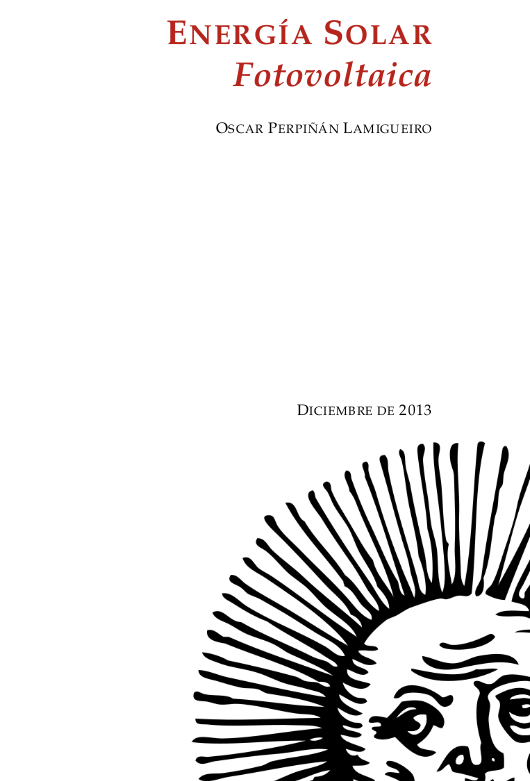
\includegraphics[width=\textwidth]{../figuras/portadaESF.png}
\end{center}
\end{block}
\end{column}
\end{columns}
\end{frame}

\section{Soluciones actuales}
\label{sec:orgf3629fb}
\begin{frame}[label={sec:org7968450}]{Soluciones actuales}
\begin{columns}
\begin{column}{0.2\columnwidth}
\begin{block}{\alert{PVsyst}}
\begin{center}

\includegraphics[width=\textwidth]{../figuras/Logo-PVsyst.png}
\end{center}
\end{block}
\end{column}
\begin{column}{0.2\columnwidth}
\begin{block}{\alert{SISIFO}}
\begin{center}

\includegraphics[width=\textwidth]{../figuras/sisifo_naranja_cab2colorpeque1.png}
\end{center}
\end{block}
\end{column}
\begin{column}{0.2\columnwidth}
\begin{block}{\alert{PVGIS}}
\begin{center}

\includegraphics[width=\textwidth]{../figuras/PVGIS.png}
\end{center}
\end{block}
\end{column}
\begin{column}{0.2\columnwidth}
\begin{block}{\alert{System Advisor Model}}
\begin{center}

\includegraphics[width=\textwidth]{../figuras/SAM-logo-horizontal.png}
\end{center}
\end{block}
\end{column}
\end{columns}
\end{frame}
\begin{frame}[label={sec:orgd6c1002},fragile]{\texttt{solaR}}
 \begin{columns}
\begin{column}{0.45\columnwidth}
\begin{block}{Funcionamiento}
\begin{itemize}
\item Geometría solar
\item Datos meteorológicos
\item Radiación en el plano horizontal
\item Radiación en el plano del generador
\item Simulación de SFCR
\item Simulación de SFB
\item Optimización de distancias
\item Métodos de visualización
\end{itemize}
\end{block}
\end{column}
\begin{column}{0.45\columnwidth}
\begin{block}{Carencias}
\begin{itemize}
\item Modularidad
\item Eficiencia y rendimiento
\item Manipulación de datos
\end{itemize}
\end{block}
\end{column}
\end{columns}
\end{frame}

\section{Marco teórico}
\label{sec:org023d9fb}
\begin{frame}[label={sec:org529f1ad}]{Procedimiento de cálculo}
\begin{center}
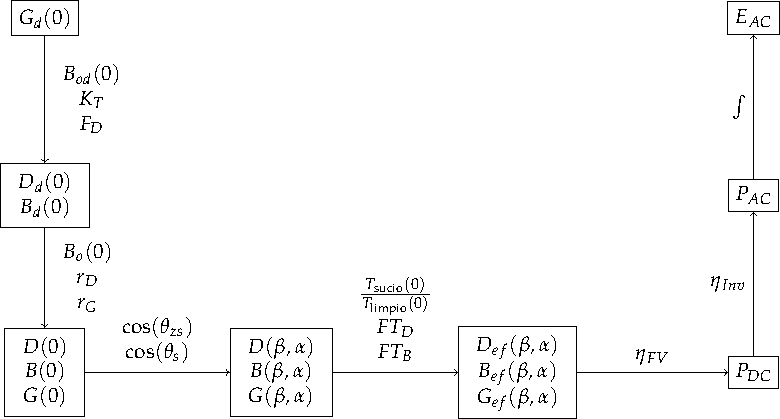
\includegraphics[scale=1]{../figuras/ProcedimientoCalculoRadiacionInclinada.pdf}
\end{center}
\end{frame}
\section{Desarrollo del código}
\label{sec:org101035a}
\begin{frame}[label={sec:org290d768}]{Algoritmo de cálculo}
\begin{center}
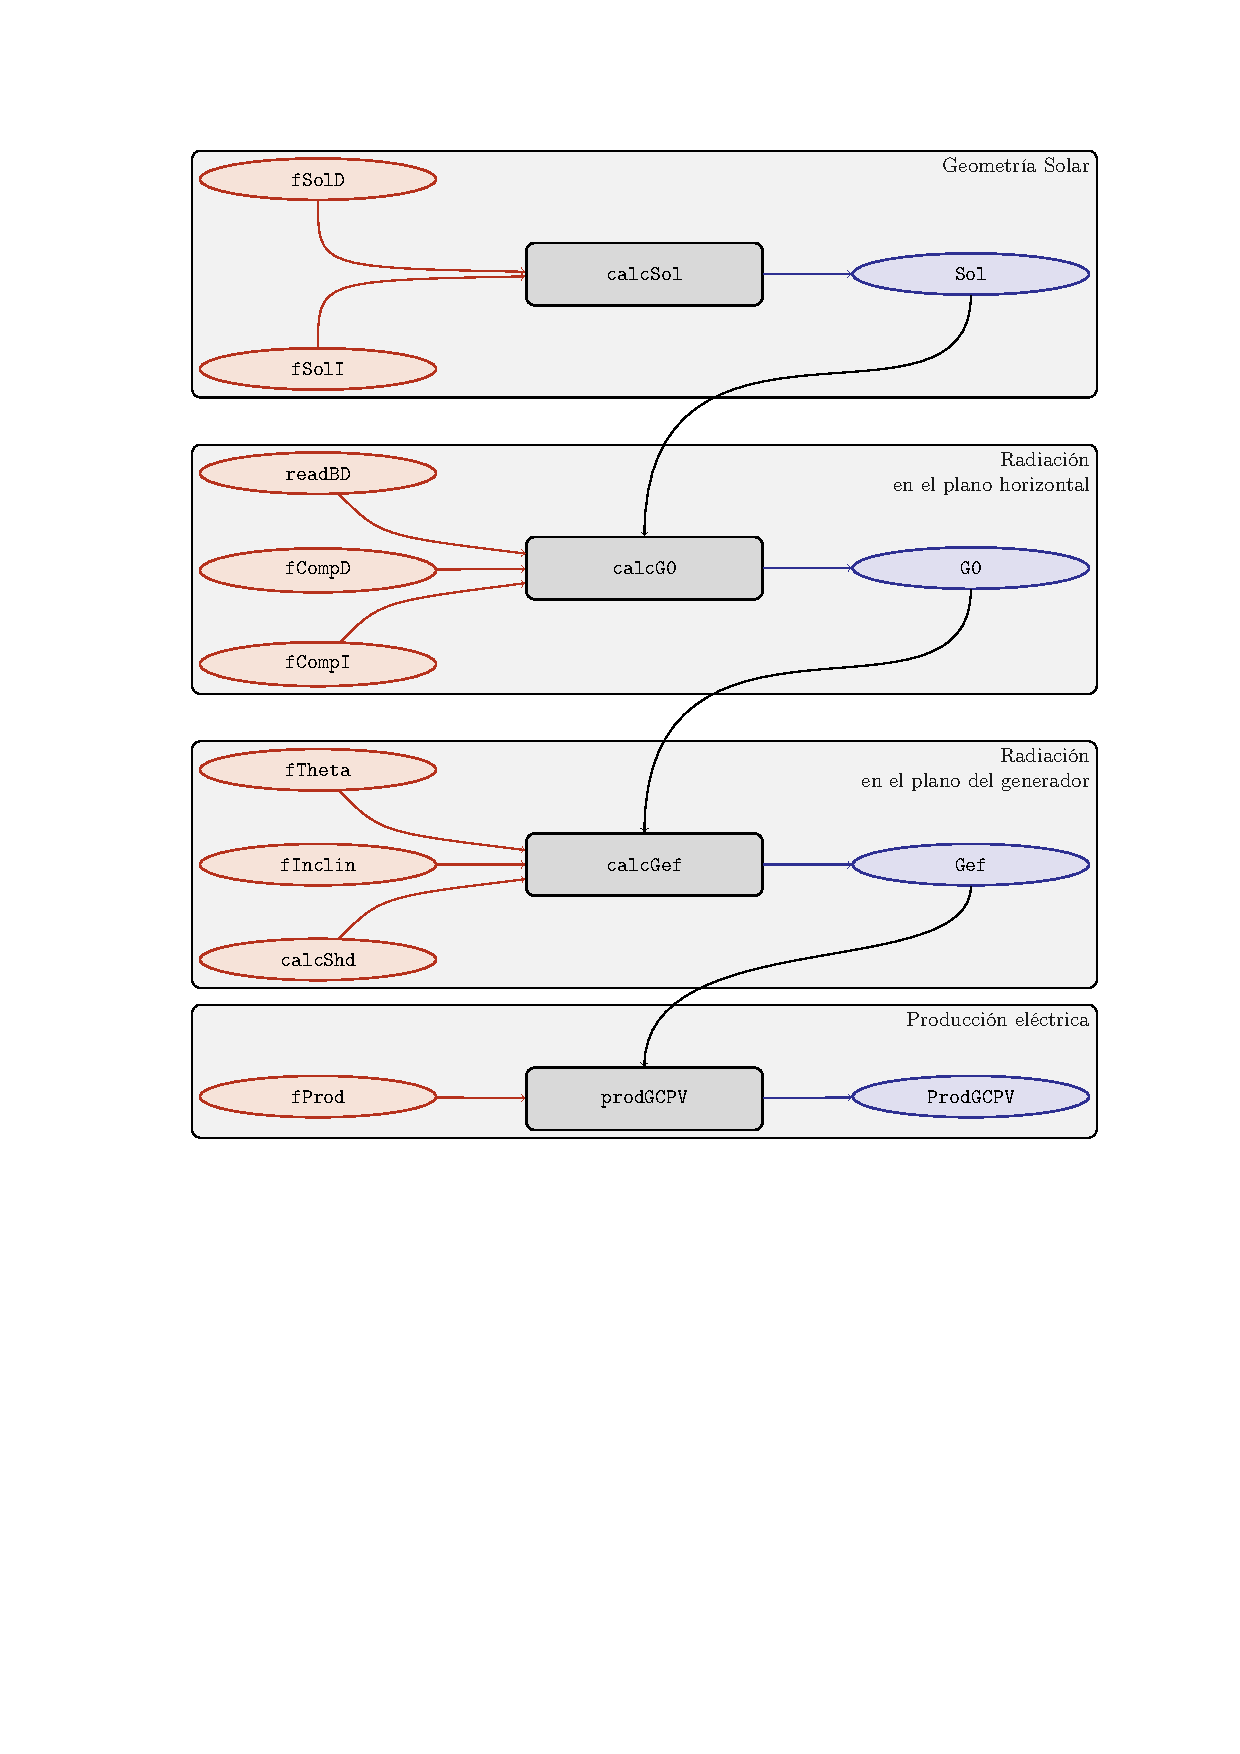
\includegraphics[height=0.9\textheight]{../figuras/procedure.pdf}
\end{center}
\end{frame}
\begin{frame}[label={sec:org2e58e8e},fragile]{\texttt{calcSol}}
 \begin{center}
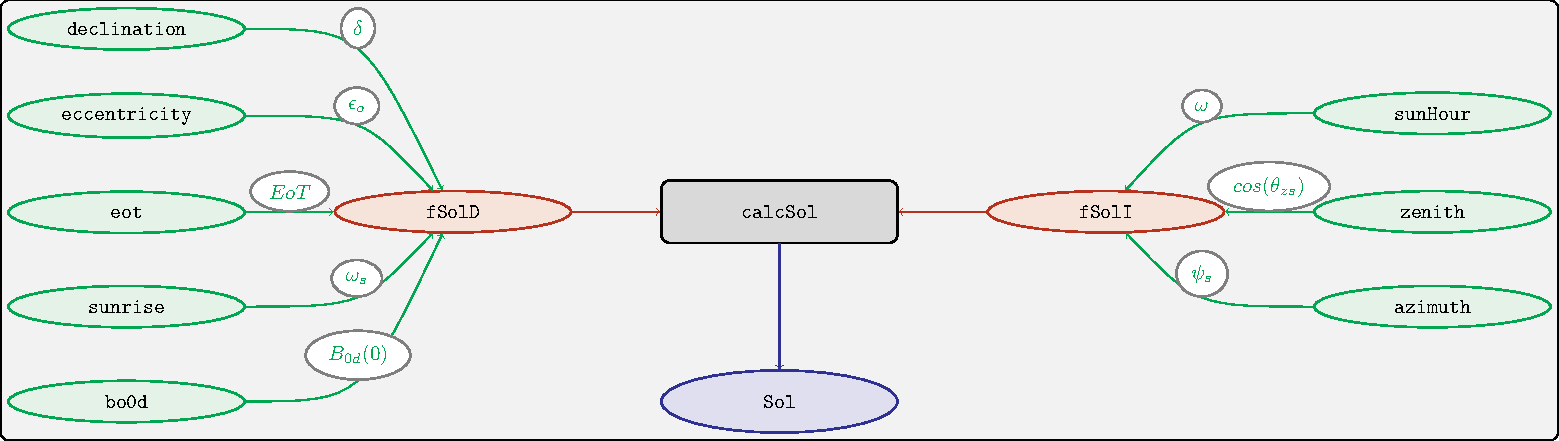
\includegraphics[width=\textwidth]{../figuras/calcsol.pdf}
\end{center}
\end{frame}
\begin{frame}[label={sec:org44433bd},fragile]{\texttt{Meteo}}
 \begin{center}
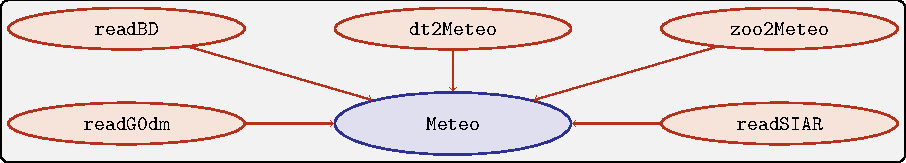
\includegraphics[width=\textwidth]{../figuras/meteo.pdf}
\end{center}
\end{frame}
\begin{frame}[label={sec:org41071cb},fragile]{\texttt{calcG0}}
 \begin{center}
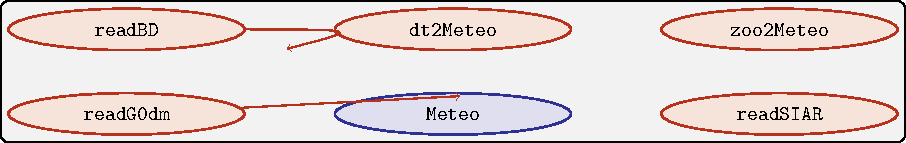
\includegraphics[width=\textwidth]{../figuras/calcg0.pdf}
\end{center}
\end{frame}
\begin{frame}[label={sec:org72253d4},fragile]{\texttt{calcGef}}
 \begin{center}
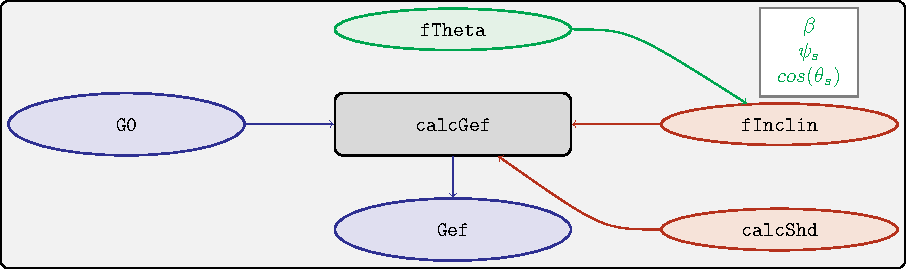
\includegraphics[width=\textwidth]{../figuras/calcgef.pdf}
\end{center}
\end{frame}
\begin{frame}[label={sec:orgc96373d},fragile]{\texttt{prodGCPV}}
 \begin{center}
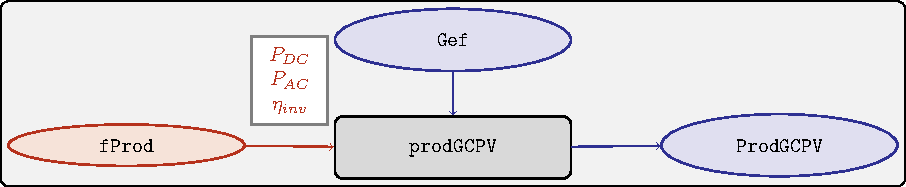
\includegraphics[width=\textwidth]{../figuras/prodgcpv.pdf}
\end{center}
\end{frame}
\begin{frame}[label={sec:orgf6e3e2a},fragile]{\texttt{prodPVPS}}
 \begin{center}
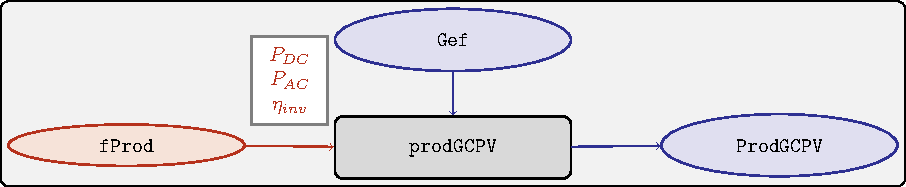
\includegraphics[width=\textwidth]{../figuras/prodpvps.pdf}
\end{center}
\end{frame}
\section{Ejemplo práctico de aplicación}
\label{sec:org00f8db9}
\begin{frame}[label={sec:org8b4ba9a},fragile]{Información meteorológica}
 \begin{lstlisting}[numbers=left,language=r,label= ,caption= ,captionpos=b]
etsidi_1315 <- readBDi(file = "TFG/data/PVGIS_1315.csv",
                       lat = 40.4, dates.col = "Dates",
                       format = "%Y-%m-%d %H:%M:%S")
\end{lstlisting}

\begin{center}
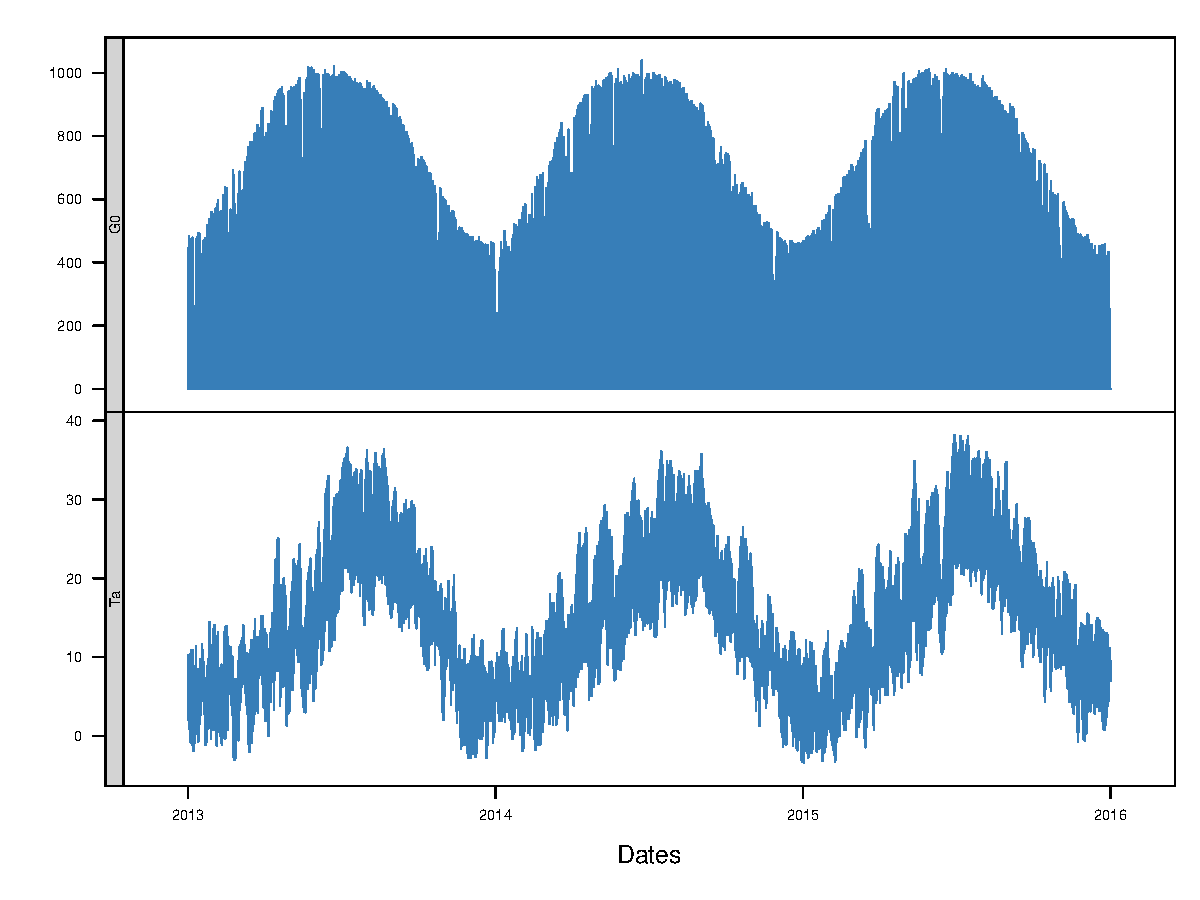
\includegraphics[width=0.5\textwidth]{../figuras/ejemplos3.pdf}
\end{center}
\end{frame}
\begin{frame}[label={sec:orgc8f2219},fragile]{Producción de diferentes sistemas}
 \begin{lstlisting}[numbers=left,language=r,label= ,caption= ,captionpos=b]
prod1 <- prodGCPV(lat = 40.4, modeTrk = 'fixed', modeRad = 'bdI',
                  dataRad = etsidi_1315, beta = 30, alpha = -19,
                  module = module1, generator = generator1,
                  inverter = inverter)
show(as.data.tableY(prod1))
\end{lstlisting}

\begin{verbatim}
   Dates      Eac      Edc       Yf
   <int>    <num>    <num>    <num>
1:  2013 1681.077 1757.235 1343.449
2:  2014 1698.613 1775.426 1357.463
3:  2015 1749.536 1828.569 1398.158
\end{verbatim}


\begin{lstlisting}[numbers=left,language=r,label= ,caption= ,captionpos=b]
prod2 <- prodGCPV(lat = 40.4, modeTrk = 'fixed', modeRad = 'bdI',
                  dataRad = etsidi_1315, beta = 30, alpha = -19,
                  module = module2, generator = generator2,
                  inverter = inverter)
show(as.data.tableY(prod2))
\end{lstlisting}

\begin{verbatim}
   Dates      Eac      Edc       Yf
   <int>    <num>    <num>    <num>
1:  2013 1451.873 1517.779 1319.225
2:  2014 1464.483 1530.833 1330.683
3:  2015 1506.544 1574.704 1368.901
\end{verbatim}
\end{frame}

\begin{frame}[label={sec:orgd288ef6}]{Comparación de producciones}
\begin{center}
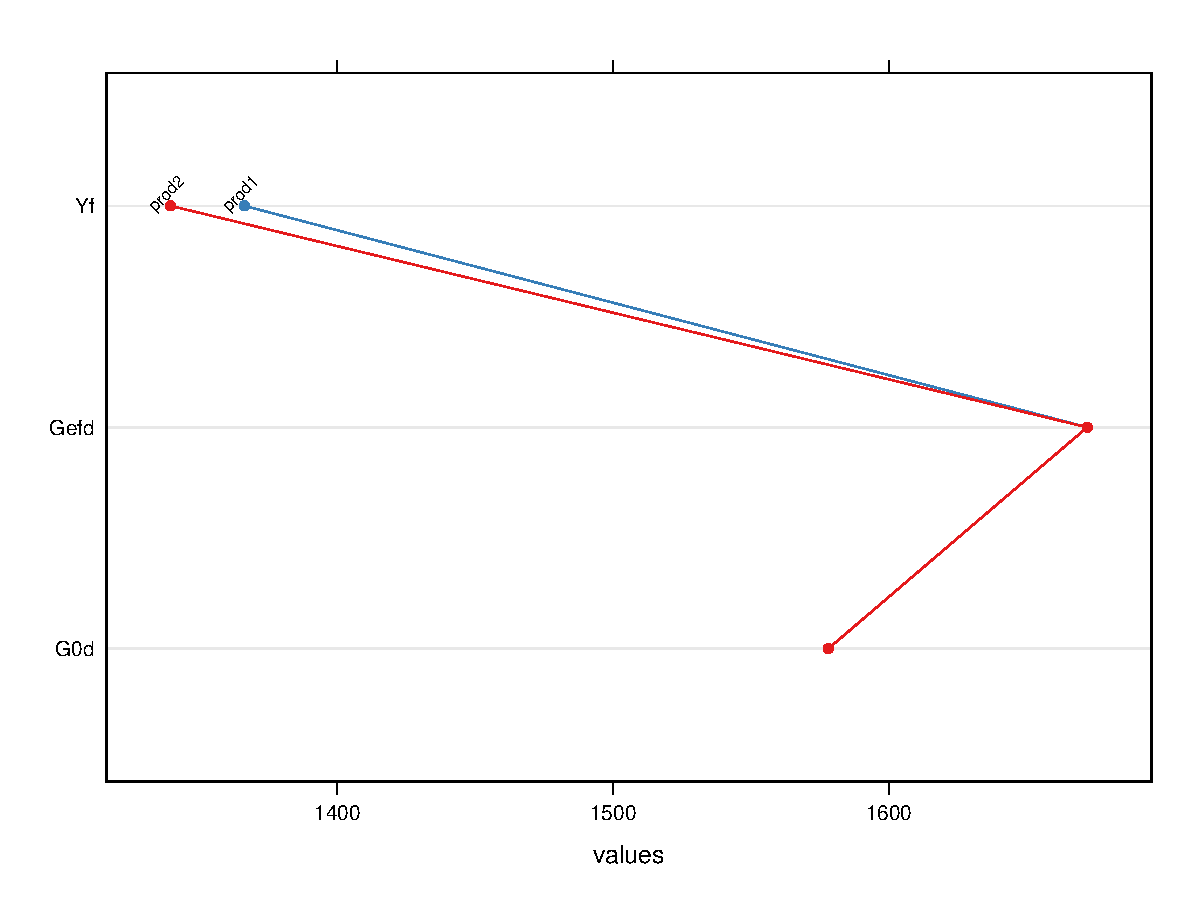
\includegraphics[height=0.9\textheight]{../figuras/ejemplos4.pdf}
\end{center}
\end{frame}
\section{Conclusiones}
\label{sec:org93e0c1c}
\subsection{Aportaciones}
\label{sec:org61584be}
\begin{frame}[label={sec:orgd3faff8}]{Blame}
\begin{center}
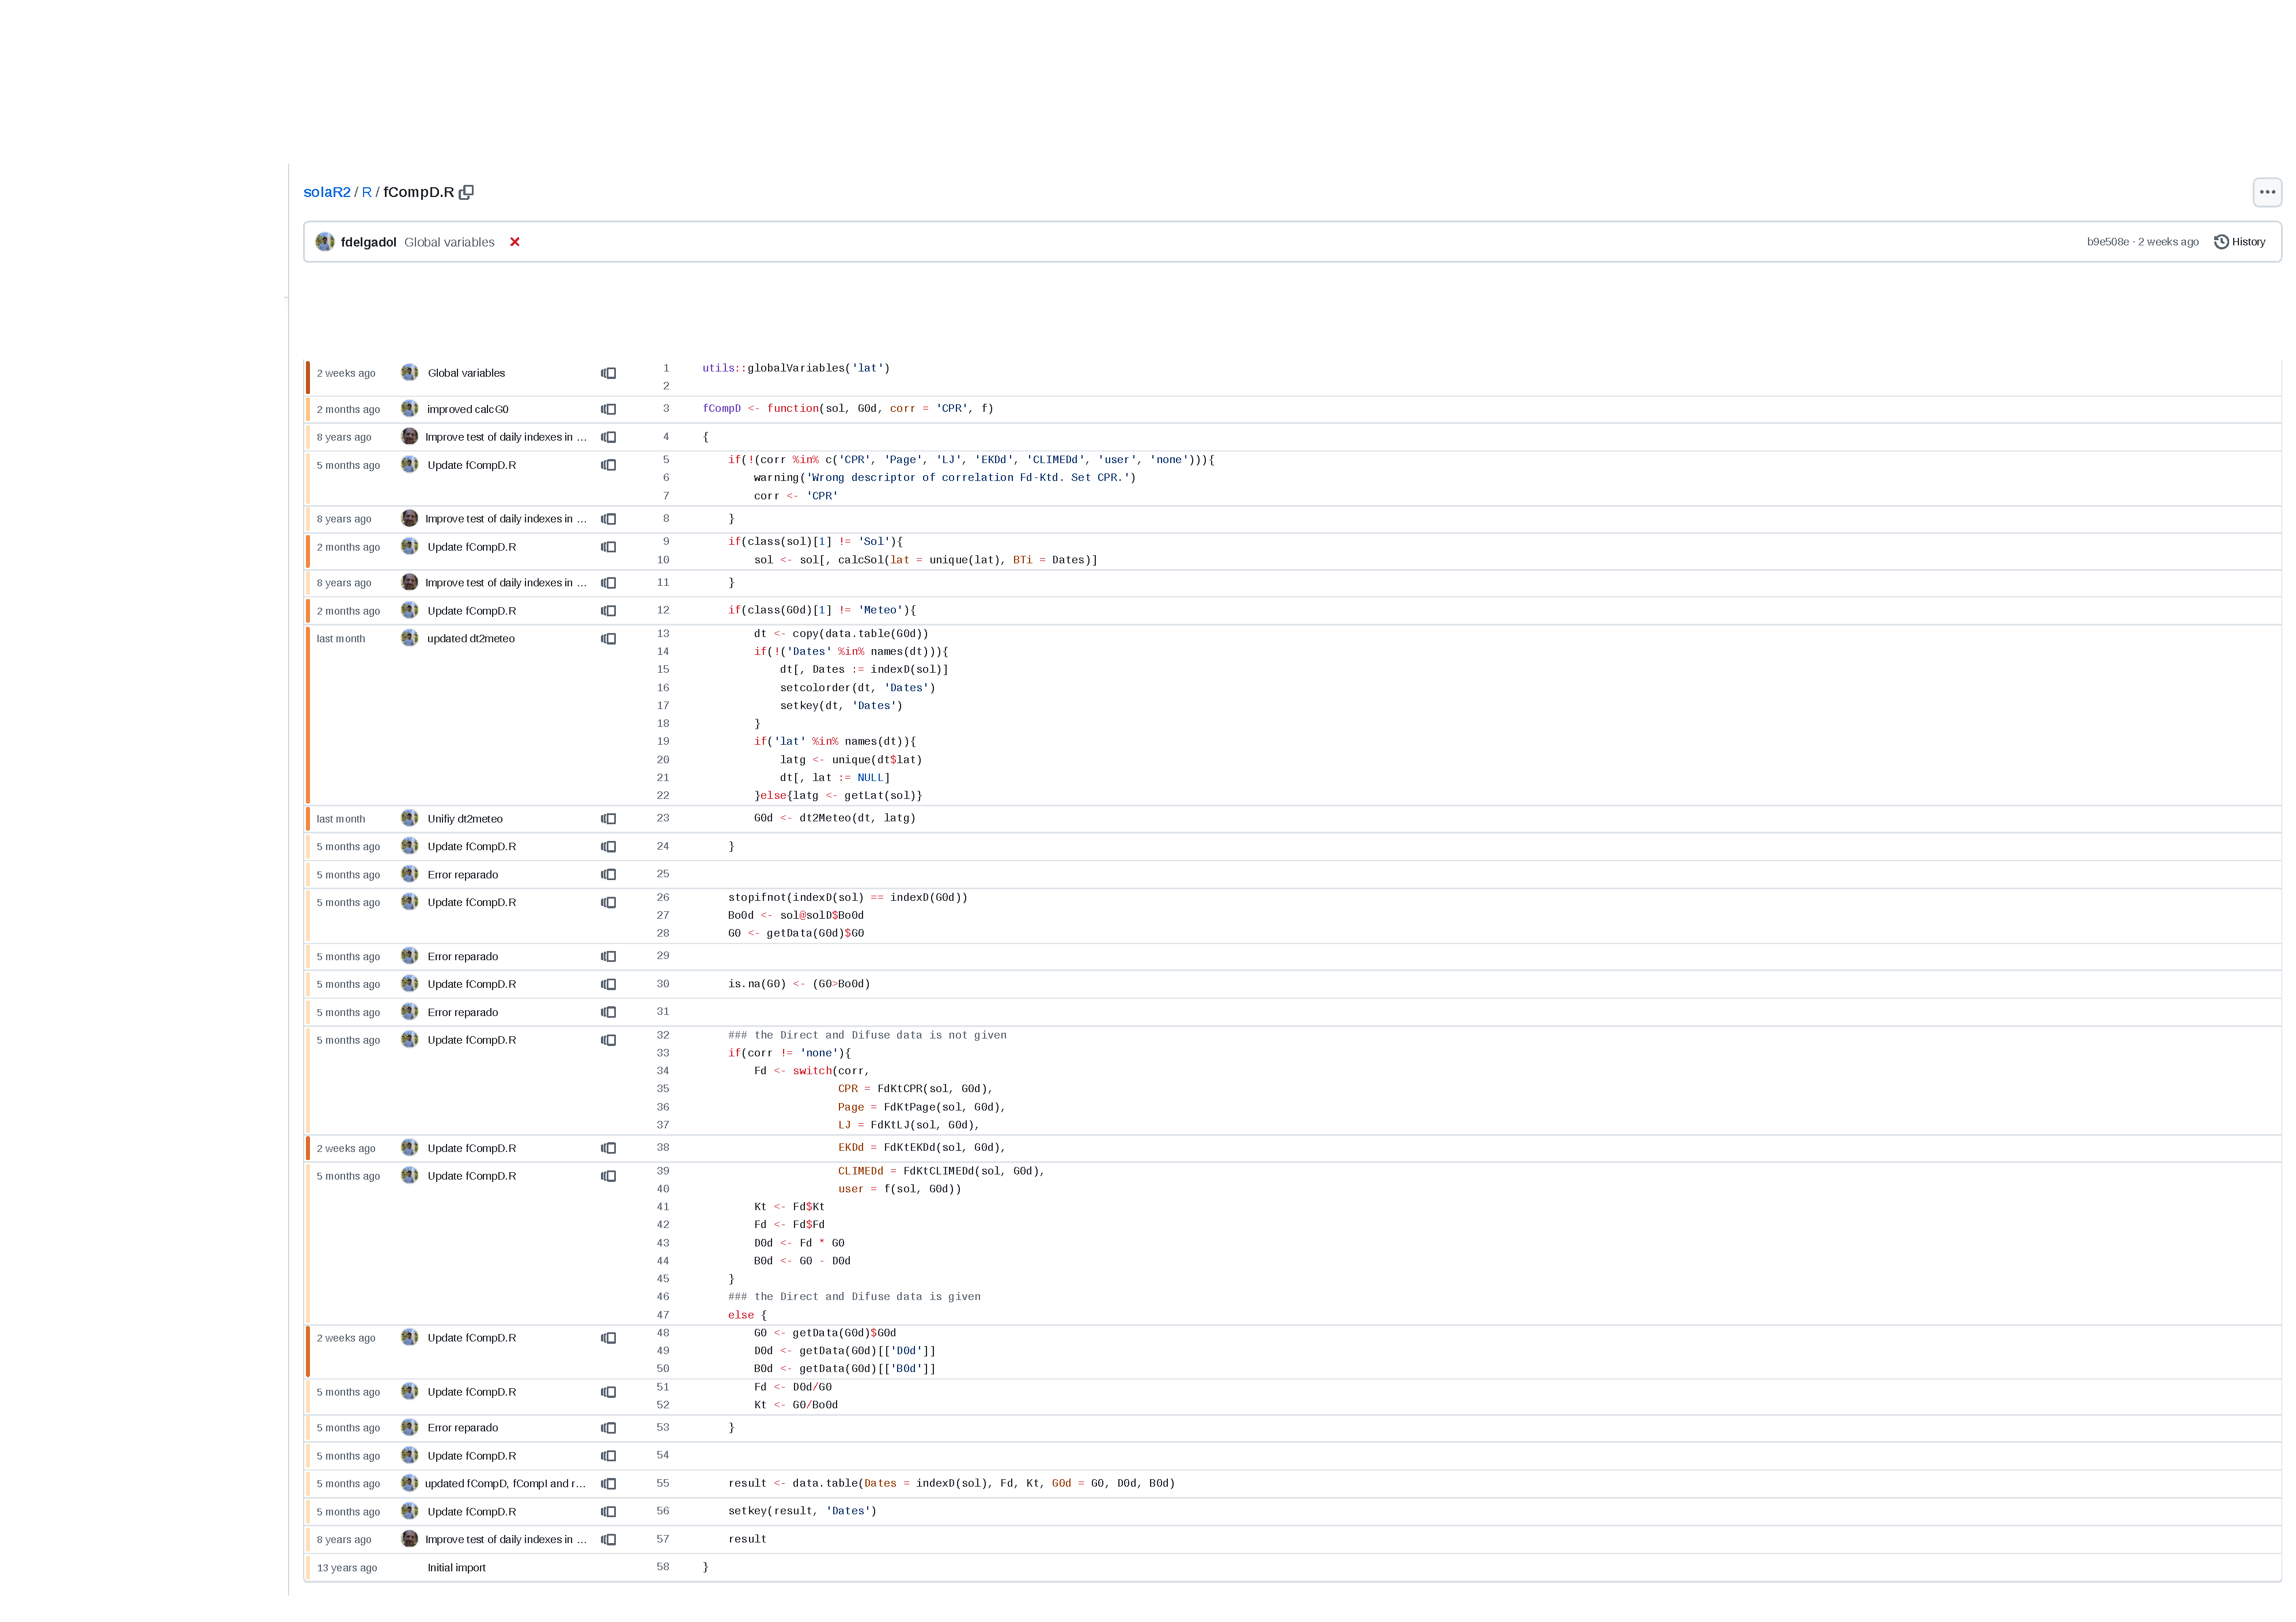
\includegraphics[height=0.9\textheight]{../figuras/blame-fCompD.pdf}
\end{center}
\end{frame}
\begin{frame}[label={sec:org862e41b}]{Blame}
\begin{center}
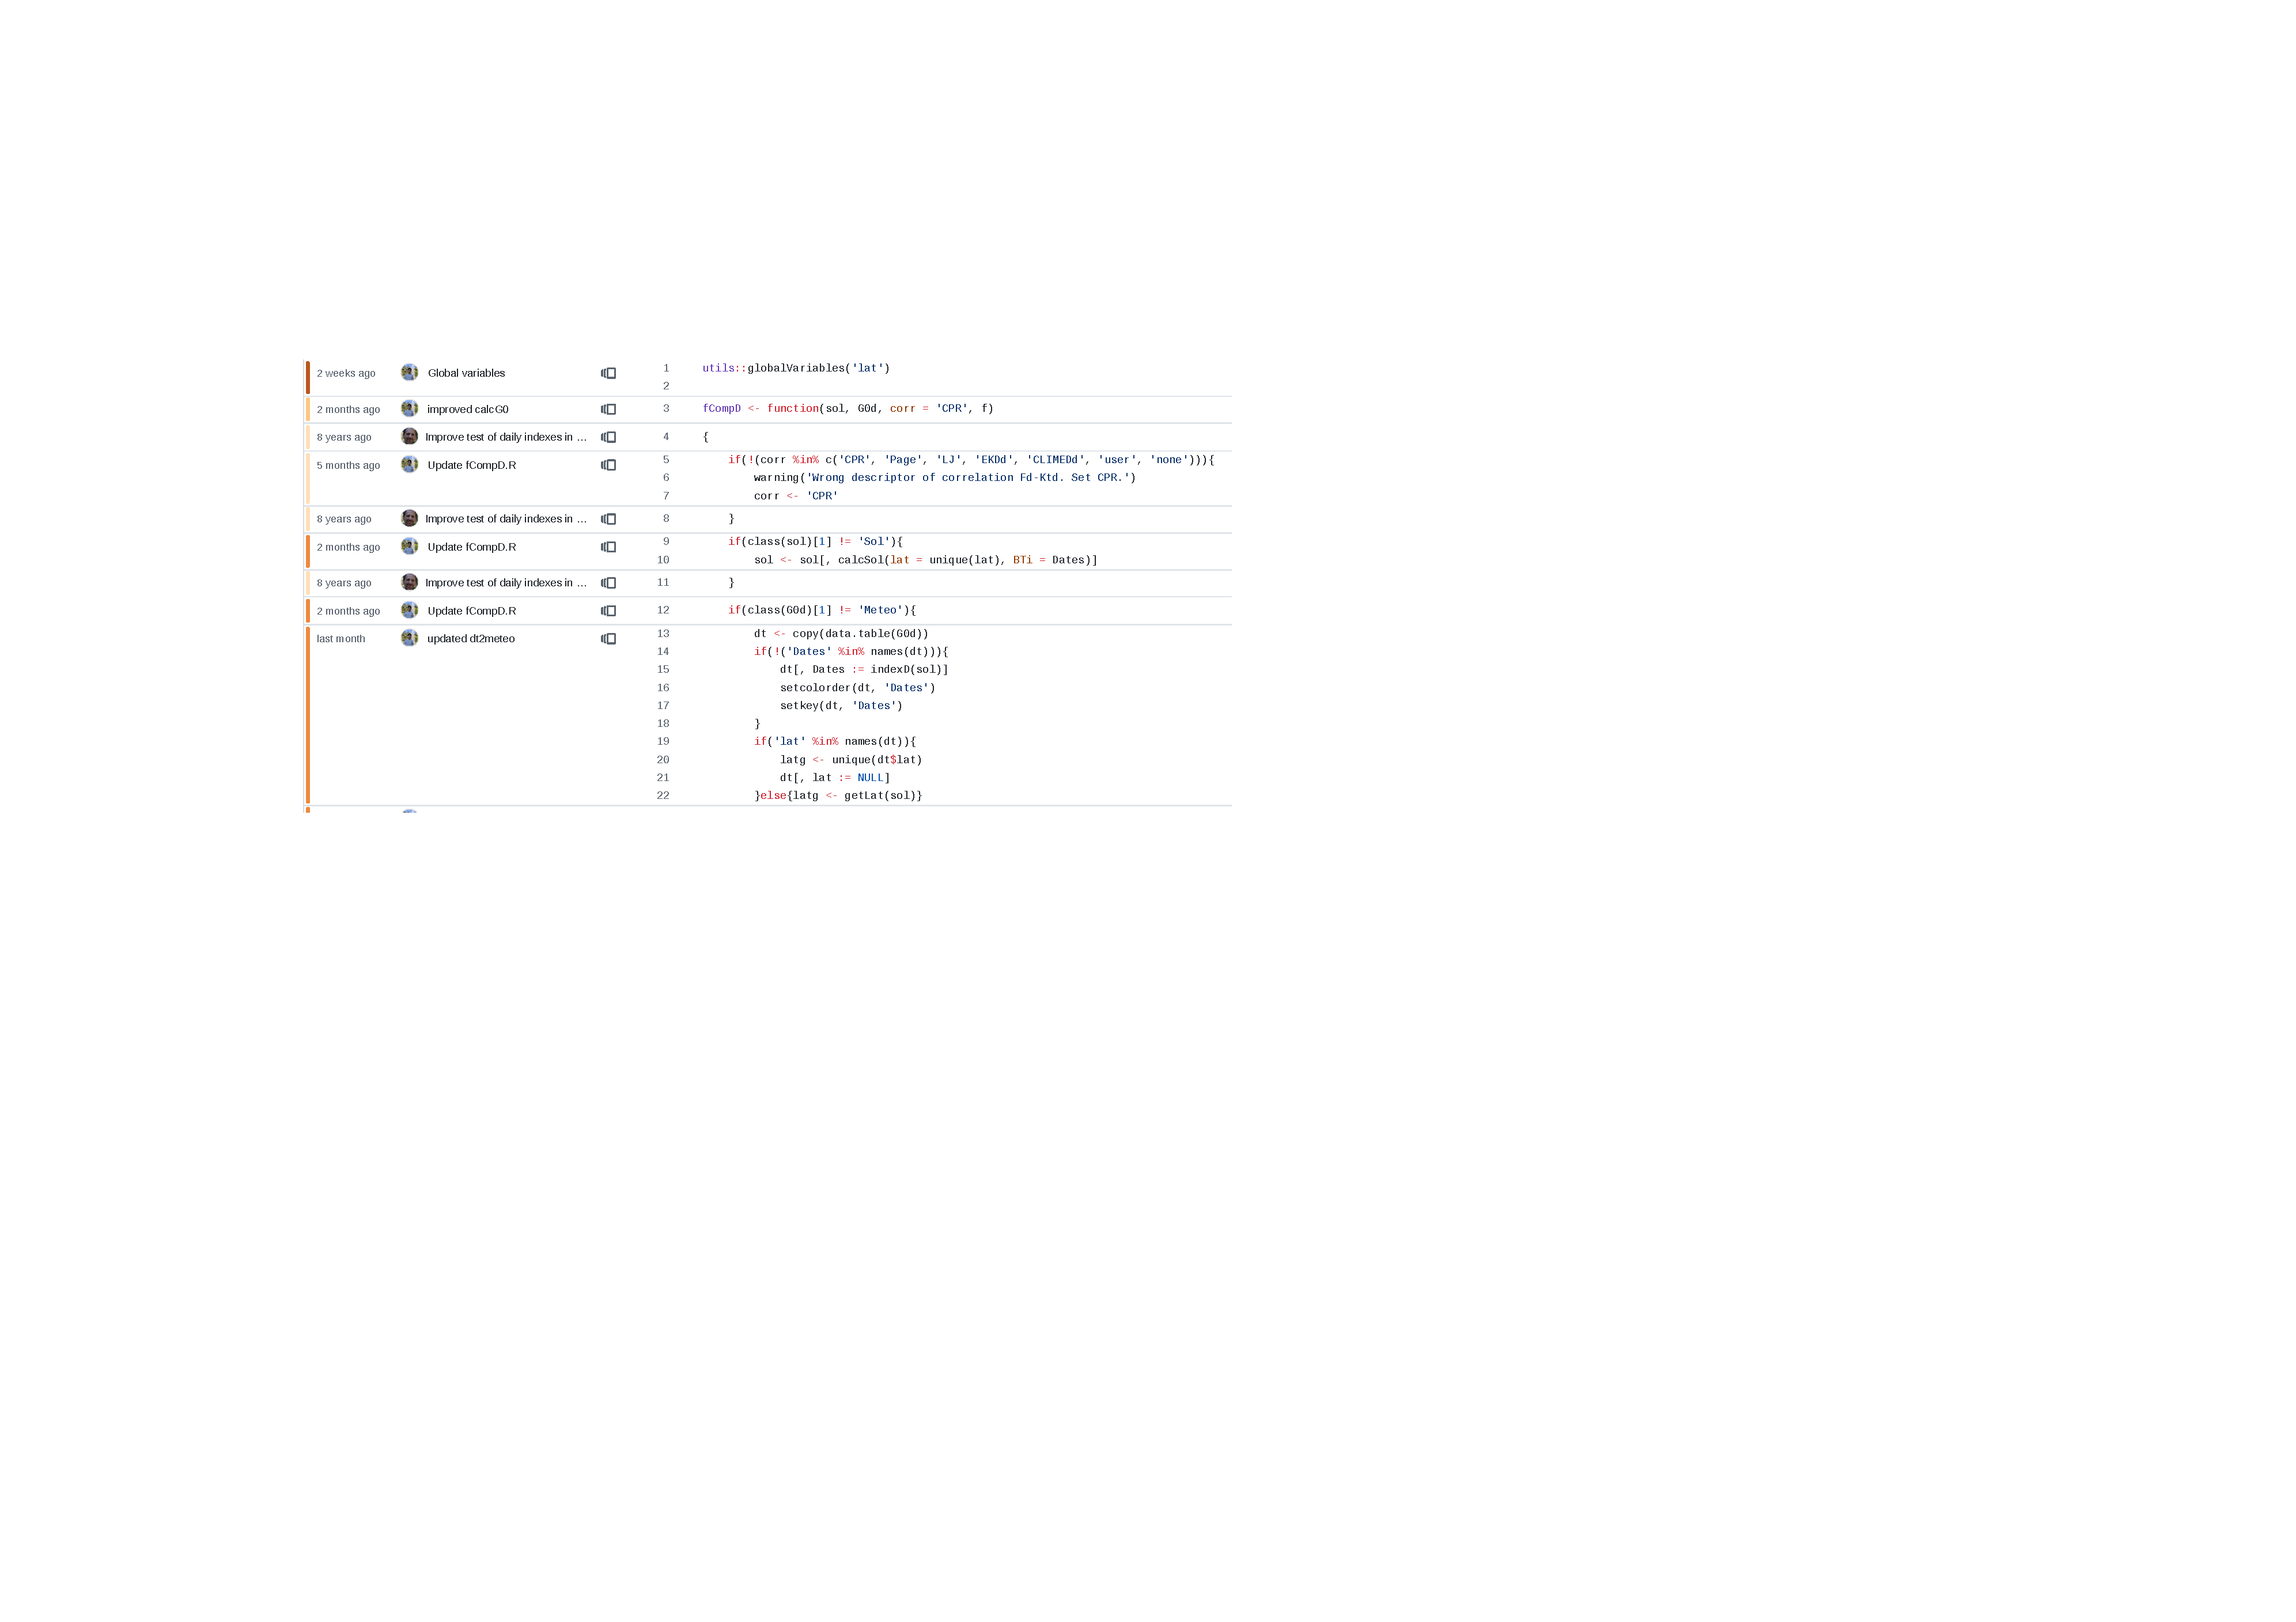
\includegraphics[width=\textwidth]{../figuras/blame-fCompD_cropped.pdf}
\end{center}
\end{frame}
\begin{frame}[label={sec:orgc49d019}]{Insights}
\begin{center}
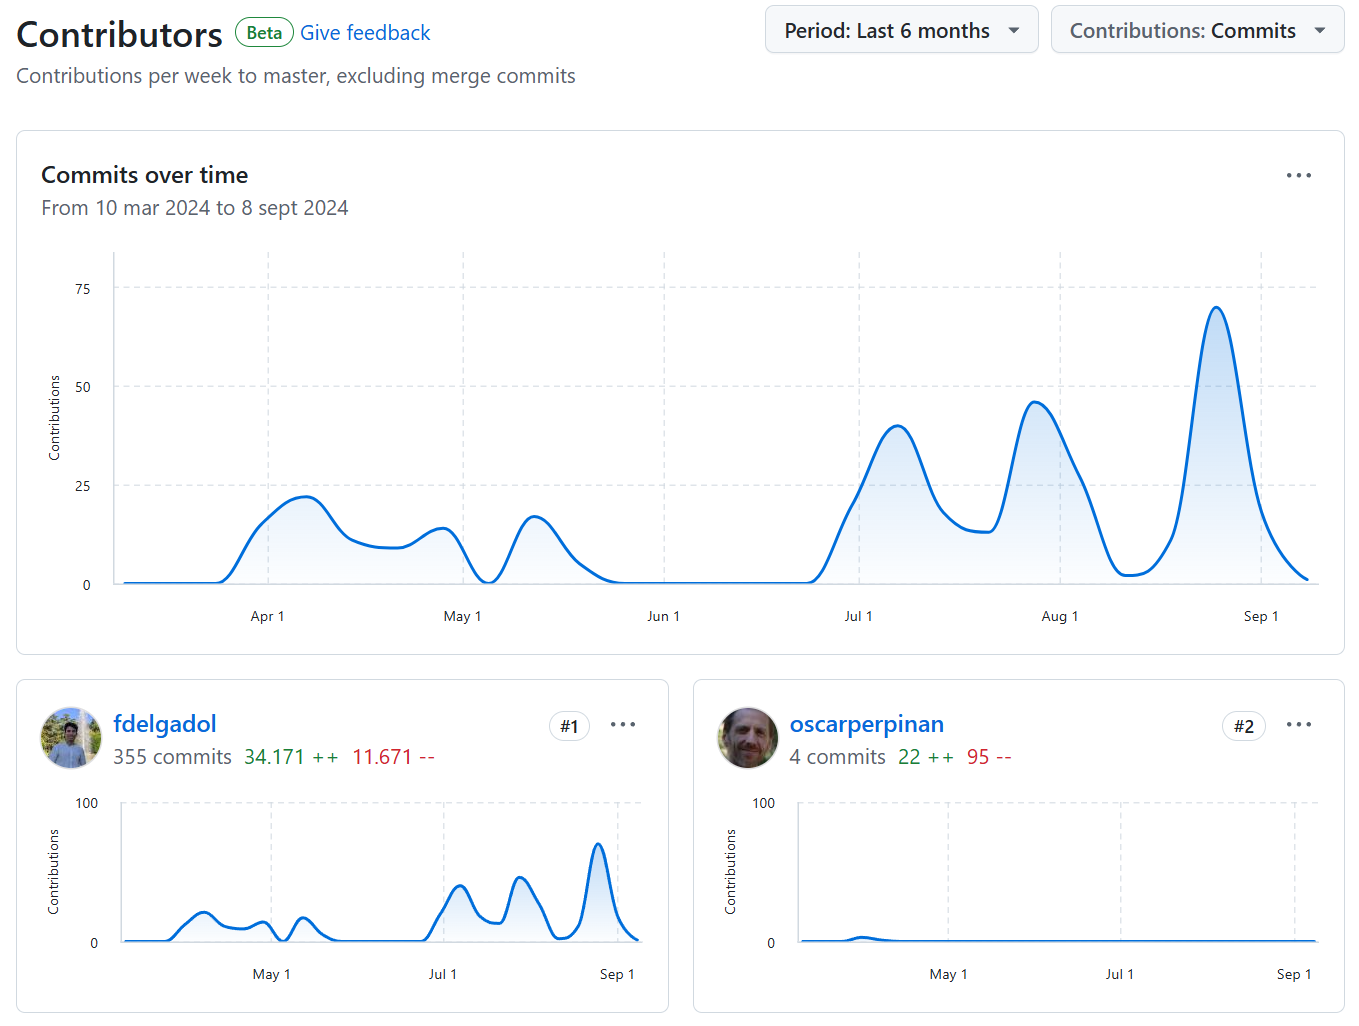
\includegraphics[height=0.9\textheight]{../figuras/contributors.png}
\end{center}
\end{frame}
\subsection{Desarrollo a futuro}
\label{sec:org091c555}
\begin{frame}[label={sec:org469f1fd},fragile]{Desarrollo a futuro}
 \begin{itemize}
\item Interfaz de usuario

\item Mejora de funciones

\item Toma de datos

\item Uso de paquete especializados en datos espaciales
\begin{itemize}
\item \texttt{terra}
\end{itemize}
\end{itemize}
\end{frame}
\subsection{Estado del paquete}
\label{sec:orga9dffd0}
\begin{frame}[label={sec:orga0dc740}]{GitHub}
\begin{center}
\href{https://github.com/solarization/solaR2}{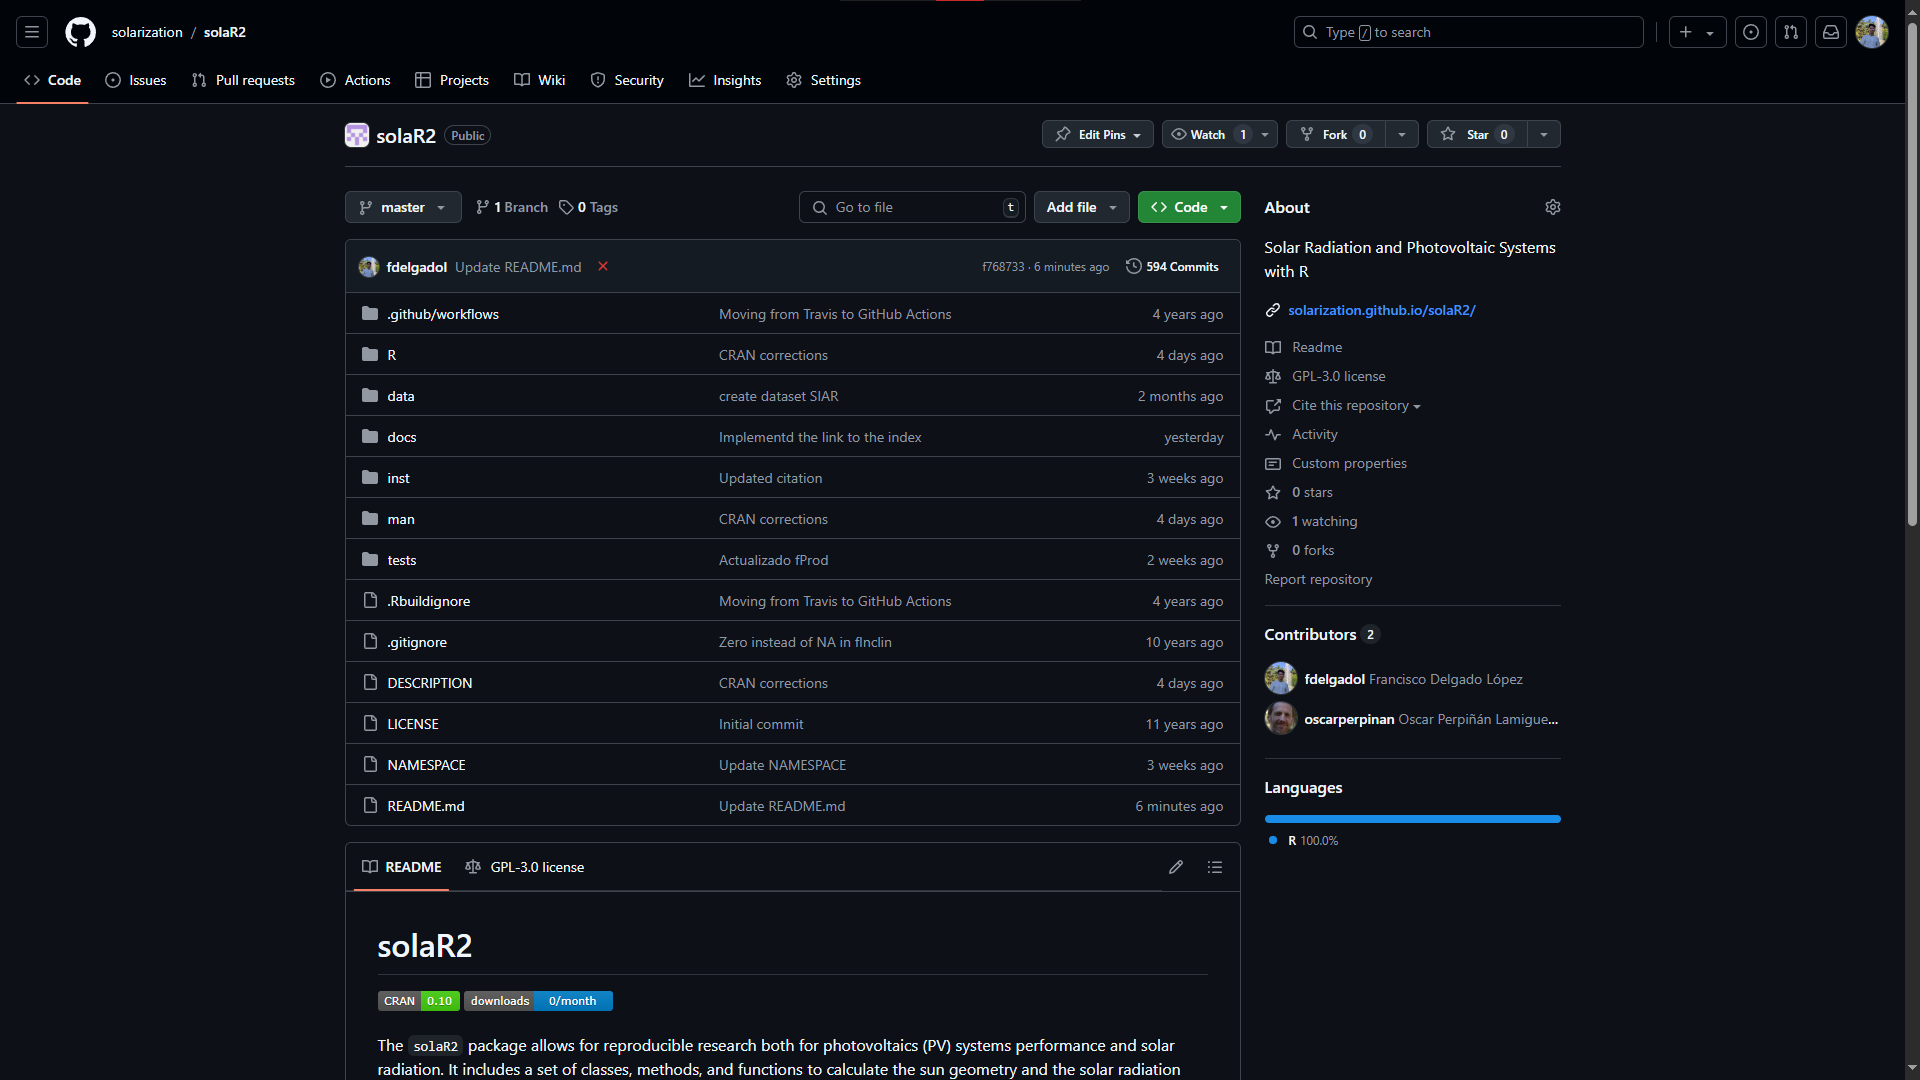
\includegraphics[width=.9\linewidth]{../figuras/GitHub.png}}
\end{center}
\end{frame}
\begin{frame}[label={sec:orgcb34332}]{CRAN}
\begin{center}
\href{https://cran.r-project.org/package=solaR2}{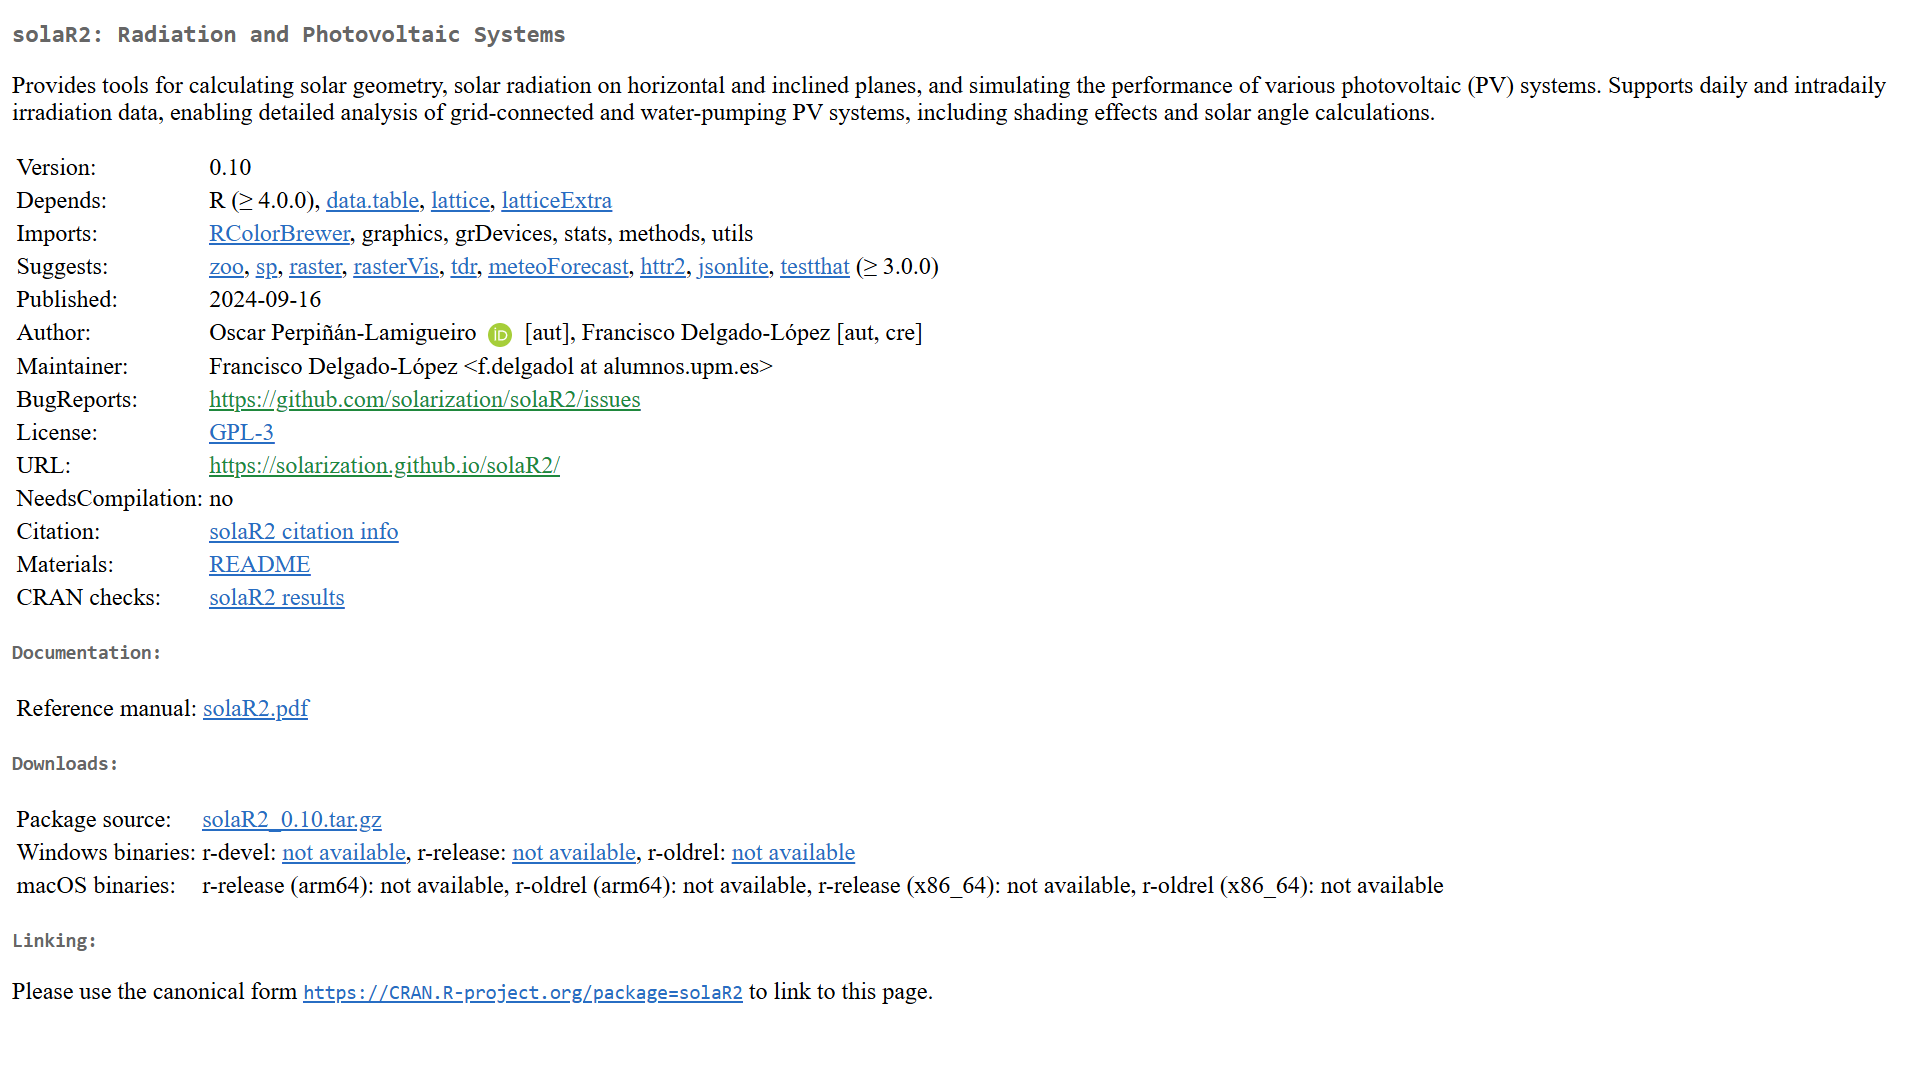
\includegraphics[width=.9\linewidth]{../figuras/CRAN.png}}
\end{center}
\end{frame}
\begin{frame}[label={sec:orgb9e27e7}]{Página web}
\begin{center}
\href{https://solarization.github.io/solaR2/}{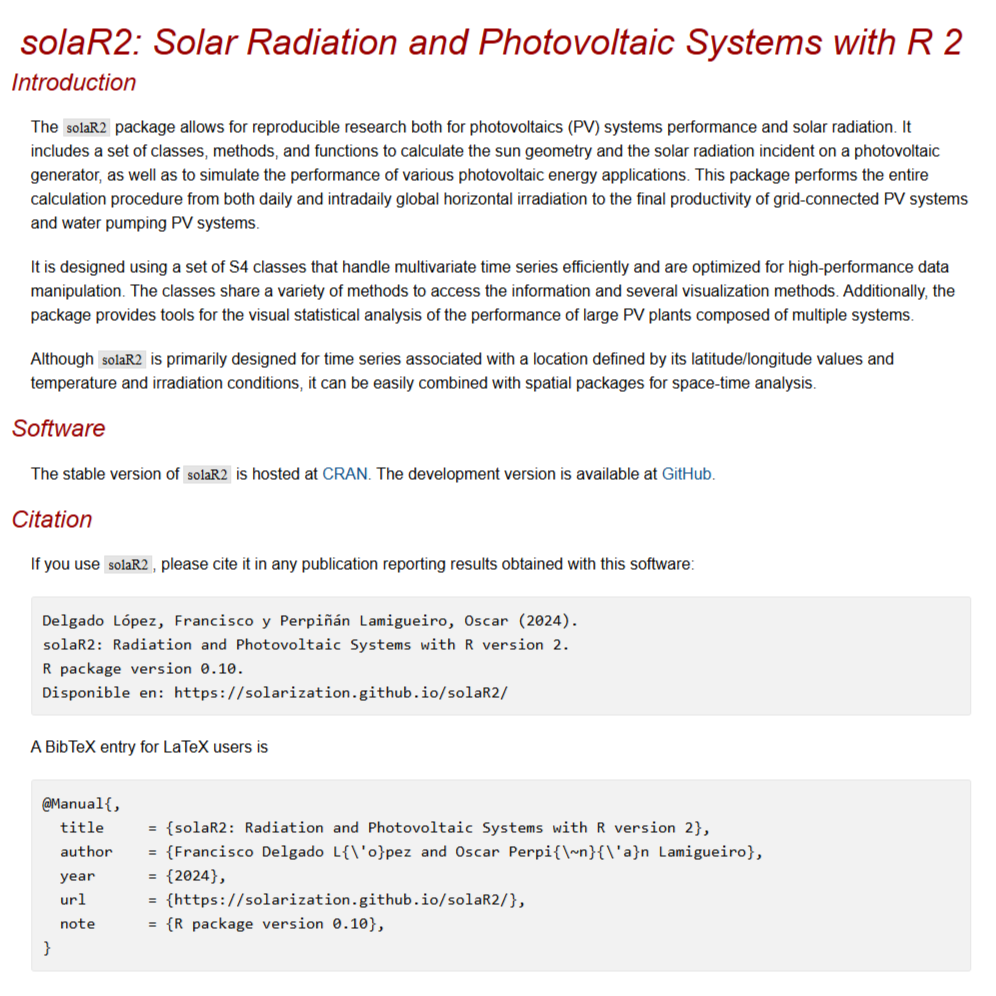
\includegraphics[height=0.9\textheight]{../figuras/github.io.png}}
\end{center}
\end{frame}
\begin{frame}[label={sec:orgf076242}]{}
\Huge
\begin{center}
\alert{Gracias por su atención}
\end{center}
\end{frame}
\end{document}
